\section{Medidas de rendimiento}

Las medidas de rendimiento de una red nos sirven para ver de manera croncreta como se comporto nuestra red, durante el entrenamiento, que fue lo que pudo aprender, que sobre aprendio, es decir, memorizo, y que aún le cuesta trabajo aprender y por tanto será incapaz de predecir. Se usan las siguientes:

\begin{description}
 \item [Matriz de confusión]: (Confusion matrix)
 Es una matriz, donde las celdas representan las predicciones que hizo nuestro modelo de clasificación de clases, respecto a las salidas esperadas. Así siendo las columnas las salidas $y$'s del modelo entrenado y las filas las salidas esperadas $y_{true}$. 
 Nos facilita a ver cuando un clasificador está condundiendo clases, contabilizando a que clase etiqueto a los diferentes ejemplares. Ahora veamos, que puede estar representando cada celda en la matriz de confusión, estos pueden ser:
 \begin{enumerate}
  \item \textbf{VP} Verdaderos positivos \emph{(TP, True Positive)}: La clasificación los ejemplares predichas, coindicen con las etiquetas esperadas de los ejemplares. 
  
  \item \textbf{VN} Verdaderos negativos \emph{(TN, True Negative)}: El ejemplar que no es parte de clase, no son asignados a ese clase, son predichos correctamente.
  
  \item \textbf{FP} Falso positivo \emph{(FP, False Positivo)}: El ejemplar que \textbf{no} es parte de una clase $i$ fue clasificado como tal.
  
  \item \textbf{FN} False negativo  \emph{(FN, False Negative)}: El ejemplar que es parte de una clase $i$ no fue clasificado como tal. 
 \end{enumerate}

  \begin{example}
   Notemos un ejemplo sencillo, supongamos que tenemos una tarea binaria, donde queremos indicar que una persona está
   embarazada (deacuerdo a unos estudios). Ahora tenemos que:

   \begin{itemize}
    \item \emph{VP}, sería predecir que una mujer está embarazada y que en efecto este embarazada. \texbf{(Correcto)}
    \item \emph{VN}, sería con un hombre que no está embarazado y pues en efecto no esta embarazado.\texbf{(Correcto)}  
    \item \emph{FP}, sería predecir que un hombre está embarazado y \texbf{no} este embarazado. \texbf{(Error, tipo 1)} 
    \item \emph{FN}, sería predecir que una mujer \texbf{no} está embarazada y este embarazada. \texbf{(Error, tipo 2)}
   \end{itemize}

   Entonces dados los resultados binarios que nos entrego el modelo, los medicos nos dan las respuestas correctas a 10
   estudios, representadas en la siguiente tabla.
 
   \begin{center}
    \rowcolors{2}{\colTableRow}{white}
     \begin{tabular}{c|cccccccccc}

      $Ejemplar$ & 1   & 2  & 3  & 4  & 5  & 6  & 7  & 8  & 9  & 10  \\ \hline
      $Sujeto$   & M   & F  & M  & F  & M  & M  & F  & F  & F  & M  \\ \hline
      $Etiqueta$ & No  & Si & No & Si & No & No & No & Si & No & No  \\ \hline
      $Clase$    & 0   & 1  & 0  & 1  & 0  & 0  & 0  & 1  & 0  & 0  \\ \hline
      $Predicho$ & 0   & 0  & 0  & 1  & 0  & 1  & 0  & 1  & 0  & 0  \\ \hline
      $Valores$  & VN  & FN & VN & VP & VN & FP & VN & VP & VN & VN  \\ \hline
   
     \end{tabular}
   \end{center}

   Con estos datos, podemos construir nuestra matriz de confusión $MC$ contabilizando las salidas obtenidas respecto a las deseadas. Quedando así de la siguiente manera:

   \begin{table}[H]
    \begin{center}
     \begin{tabular}{|c|c|c|c|}
     \cline{3-4}
     \multicolumn{2}{c|}{} & \multicolumn{2}{c|}{Salidas $y$} \\
     \cline{3-4}
     \multicolumn{2}{c|}{} & Si & No \\
     \hline
     \multirow{3}{*}{Etiquetas} & Si & $VP = 2$ & $FN = 1$ \\
     \cline{2-4}
     & No & $FP=1$ & $VN = 6$  \\
     \hline
     \end{tabular}
    \end{center}
    \caption{Matriz de confusión binaria.}
    \label{Table2}
   \end{table}

\label{ej:binario}
\end{example}
 
 
 Ahora para una modelo que sea multiclase, en el que tengamos que clasificar varias clases de ejemplares. Tendremos una matriz $M$ de $n * n$ donde $n$ es el número de clases, así los valores \emph{VP, VN, FP, FN}, son calculados para cada clase e identificados en la matriz $M$ de la siguiente forma, también puedes ver la figura \ref{fig:mcMult}:
 \begin{itemize}
  \item \emph{VP}, para la clase $i$ será la celda $M[i][j]$ con la $i = j$.
  
  \item \emph{VN}, para la clase $i$ será la suma de los valores de toda la matriz menos los valores de la fila $i$ ni los valores de la columna $i$. 
  
  \item \emph{FN}, para la clase $i$ será la suma de los valores en la fila $i$, excepto la celda $M[i][j]$, con $i=j$ que es el \emph{VP}.
  
  \item \emph{FP}, para la clase $i$ será la suma de los valores en la columna $i$, excepto la celda $M[i][i]$ que es el \emph{VP}.
 
 \end{itemize}
 
  \begin{figure}[H]
 \centering
 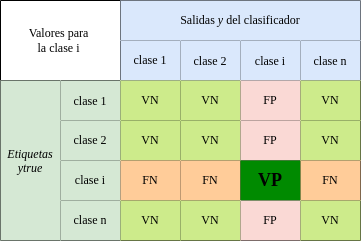
\includegraphics[scale=0.7]{../Figuras/MC_multiple.png}
 \caption{Matriz de confunsión para clasificador multiclases.}
 \label{fig:mcMult} 
\end{figure}

 
 \begin{example}
Tenemos un clasificador encargado de identificar las cinco vocales del español, escritas a mano. Entonces tenemos un total de 5 clases representadas por $a, e, i, o, u$, cada letra representada por un número del 0 al 4. Así la clase $0 = a$, la clase $1 = e$ y así respectivamente. Este fue entrenado con 15 ejemplares etiquetados y se obtuvieron los siguientes resultados:


\begin{center}
\rowcolors{2}{\colTableRow}{white}
\begin{tabular}{c|ccccccccccccccc}

 $Ejemplar$ $e$     & 1 & 2 & 3 & 4 & 5 & 6 & 7 & 8 & 9 & 10 & 11 & 12 & 13 & 14 & 15 \\ \hline
 $Etiqueta $      & a & e & i & o & u & a & a & e & i & i  & o  & u  & o  & u & a \\ \hline
 $Clase$ $y_{true}$ & 0 & 1 & 2 & 3 & 4 & 0 & 0 & 1 & 2 & 2  & 3  & 4  & 3  & 4 & 0 \\ \hline
 $Predicho$ $y$     & 0 & 1 & 3 & 3 & 2 & 1 & 1 & 1 & 2 & 2  & 4  & 4  & 3  & 2 & 0 \\ \hline

\end{tabular}
\end{center}
\end{example}

 Ahora para hacer la matriz de confusión $MC$ notamos que tenemos una matriz de $5 x 5$, donde $MC[i]= Predicho$ y $MC[][j] = EtiquetasReales$. Entonces necesitamos contabilizar las predicciones y asignarlas a su respectivas celdas, donde con la tabla anterior notamos que en el ejemplar $e3$ con $y_{true}(e3)= 2$, se predijo que $y(e3)=3$, entonces $MC[2][3] +=1$, pues la etiqueta nos pocisiona en la fila $2$ y lo predicho en la columna $3$. Ahora en el ejemplar $e4$ con $y_{true}(e4)= 3$ se predijo que $y(e4)= 3$, entonces  $MC[2][2] +=1$. Así con cada ejemplar vamos a ir sumando su clasificación. Para construirla tendriamos un pseudocódigo siguiente:
 \begin{verbatim}
  def getMC (Ejemplares, y):
      """
      :param y:  salidas obtenidas (int)
      """
      MC = [len(y)][len(Ejemplares] # y == Ejemplares
      full_zeros(MC)
      for e in range (0, len(Ejemplares)):
          predicho = y[e]
          y_true = Ejemplares[e].etiqueta
          MC[predicho][y_true] += 1
  retrun MC
 \end{verbatim}

Dados los datos anteriores tenemos, la siguiente matriz de confusión: 
 \begin{table}[H]
\begin{center}
%\rowcolors{2}{\colTableRow}{white}
\begin{tabular}{|c|c|c|c|c|c|c|c|}
\cline{3-8}
\multicolumn{2}{c|}{} & \multicolumn{5}{c|}{Salidas $y$} \\
\cline{3-8}
\multicolumn{2}{c|}{} & 1 & 2 & 3 & 4 & 5 \\
\hline
\multirow{5}{*}{\begin{sideways} Etiquetas~ \end{sideways}} & 1 & $2$ & $2$ & $0$ & $0$ & $0$ \\
\cline{2-8}
& 2 & $0$ & $2$  & $0$ & $0$ & $0$ \\
\cline{2-8}
& 3 & $0$ & $0$  & $2$ & $1$ & $0$ \\
\cline{2-8}
& 4 & $0$ & $0$  & $0$ & $2$ & $1$ \\
\cline{2-8}
& 5 & $0$ & $0$  & $2$ & $0$ & $1$ \\
\hline
\end{tabular}
\end{center}
\caption{MC = Matriz de confusión multiclase.}
\label{Table2}
\end{table}

\label{ej:binario}
\end{example}
 

 Para calcular los valores \emph{VP, VN, FP,FN}, por clase se propone el siguiente pseudocodigo:
 \begin{verbatim}
  MC = getMC(y_salidas, y_true)
  
  VP = VN = FP = FN = [0,0,0,0,0]

  for i in range(len(MC)):
    for j in range(len(MC[0])):
        FN[i] = FN[i] + MC[i][j] if (i != j) else FN[i]
        FP[i] = FP[i] + MC[j][i] if (i != j) else FP[i]
        VP[i] = MC[i][j] if (i == j) else VP[i]
    VN[i] = sum(MC) - FN[i] - FP[i] -VP[i]
 \end{verbatim}

 Si quisieramos saber los valores \emph{VP, VN, FP,FN}, para todo el desempeño total, simplemente sumamos lo obtenido en cada clase así:

 \begin{verbatim}
  VP_total = sum(VP)
  VN_total = sum(VN)
  FP_total = sum(FP)
  FN_total = sum(FN)
 \end{verbatim}

    Ahora los valores de cada celda nos representan lo siguiente:
 
   \begin{itemize}
     \item \emph{$VP_{total}$}, toda la diagonal de la matriz. La salida del modelo coincide con lo etiquetado con el ejemplar.
     \item \emph{$VN_{total}$}, todas las veces que no era la clase i y dijo que no era de la clase i.
     \item \emph{$FN_{total}$}, todas las veces que era $clase_{i}$ y dijo que era $clase_{x}$. (deseado $FN = 0$ )
     \item \emph{$FP_{total}$}, todas las veces que predijo que era $clase_{i}$ y era $clase_{x}$. (deseado $FP = 0$ )
   \end{itemize}
 
    Así que, si los valores que no estan en la diagonal de la matriz son cero o todas nuestras clasificaciones están en la diagonal, podemos decir que nuestro modelo aprendio a clasificar correctamente todas las clases.
 
 \end{description}
\begin{description}

 \item [Precisión y recupecación (recall)]: Para saber que tan presisa fue nuestro modelo se usa la equación P, y para saber que tanto se equivoco la ecuación R. Descritas acontinuación:
    \begin{equation}
        P = \dfrac{VP}{VP+FN} 
    \end{equation}
    \begin{equation}
        R = \dfrac{VP}{VP+FP} 
    \end{equation}
    
    \begin{itemize}
     \item Cuando el modelo detecta los ejemplares pero los incluye en otras clases también: \emph{P} es bajo y \emph{R} es alto. 
     \item Cuando el modelo no detectó bien los ejemplares pero tampoco los incluyo en otras clases: \emph{P} es alto y \emph{R} es bajo. 
     \item Cuando el modelo detecta los ejemplares y no los incluye en tras clases:\emph{P} y \emph{R} es alto. 
     \item Cuando el modelo no detecta los ejemplares:\emph{P} y \emph{R} es bajo. 
     \end{itemize}

 \item [Exactitud (accurrancy) y f (f score)]: La accurrancy es para ver que tan cerca estuvimos de identificar los valores esperados (no se recomienda usar si tienes clases desbalancedas, es decir, muchos elementos de una clase y poco de otra pues nos puede fallar totalmente con las clases pequeñas y aún así su valor sería alto). La \emph{f} se utiliza para combinar las medidas de precision y recall en un sólo valor. Es práctico porque hace más fácil el poder comparar el rendimiento combinado de la precisión y la recall entre varias soluciones. Se dan las ecuaciones acontinuación:
    
    \begin{equation}
     A = \dfrac{VP+VN}{VP + VN + FP + FN} = \dfrac{VP+VN}{Todos los valores clasificados}     
    \end{equation}

    \begin{equation}
     F = \dfrac{2}{\dfrac{1}{P} +\dfrac{1}{R} }= 2 \dfrac{P * R}{P + R}
    \end{equation}


